\documentclass{beamer}
\usepackage[T1]{fontenc}
\usepackage{textcomp}
\usepackage[utf8x]{inputenc}
\usepackage[british]{babel}
\usepackage{url}
\usepackage{listings}
\usepackage{graphicx}
%\usepackage{multicol} 

\usepackage{booktabs}
%\usepackage{soul}

%FONT
\usepackage{bera}
\usepackage[garamond]{mathdesign}
\renewcommand{\rmdefault}{ugm} % garamond
\renewcommand{\sfdefault}{ugm} % sans-serif font


\title{Fitting an All-atom Protein Model to a $C_{\alpha}$-trace}

\author{\small Martin Dybdal \and Anders Boesen Lindbo Larsen \and Esben Skaarup}

\institute{\textrm{Datalogisk Institut, Københavns Universitet}}
\date{\today}

\mode<presentation>
{
  \usetheme{Frankfurt}
  %\usetheme{Warsaw} 
  \definecolor{uofsgreen}{rgb}{.125,.5,.25}
  \definecolor{natvidgreen}{rgb}{.196,.364,.239}
  \definecolor{kugrey}{rgb}{.4,.4,.4}
  \usecolortheme[named=uofsgreen]{structure}
  \usefonttheme[onlylarge]{structuresmallcapsserif}
  \usefonttheme[onlysmall]{structurebold}
}

\logo{
\includegraphics[height=1.5cm]{diku.png}}

\usenavigationsymbolstemplate{} % fjern navigation

\setcounter{tocdepth}{1}

\begin{document}

\frame{\titlepage}

% Martin
\section{Introduction}
\subsection{Protein structure}

\begin{frame}[t, fragile]
  \frametitle{Protein Structure Prediction}
  
\end{frame}

\begin{frame}[t, fragile]
  \frametitle{From $C_\alpha$-trace to an all-atom model}
  \begin{columns}
    \column{5cm}
  \begin{figure}
    \centering
    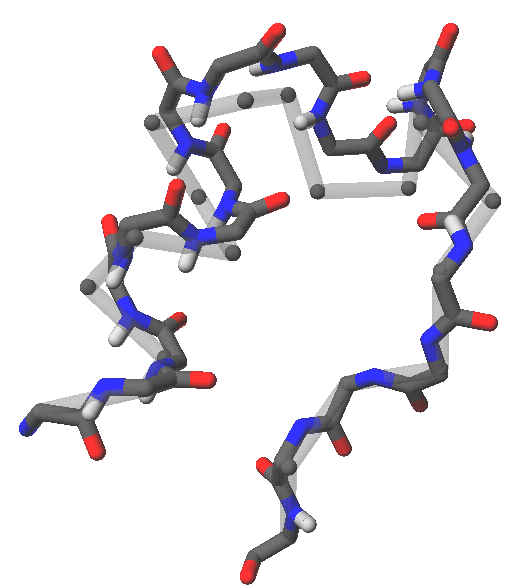
\includegraphics[width=\textwidth]{../rapport/figures/forside.png}
    \caption{Fitting of an all-atom model to a $C_\alpha$-trace}
    \label{fig:front}
  \end{figure}

  \column{5cm}

  \begin{figure}
    \centering
    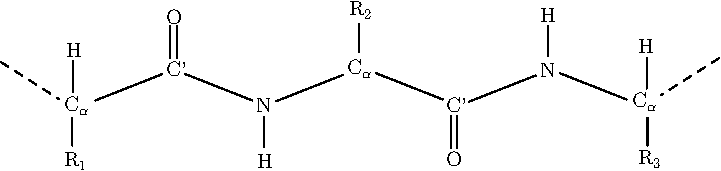
\includegraphics[width=\textwidth]{../rapport/figures/amino_connect.pdf}
    \caption{All-atom model}
    \label{fig:front}
  \end{figure}

  \begin{figure}
    \centering
    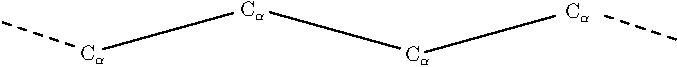
\includegraphics[width=\textwidth]{../rapport/figures/Calpha_backbone.pdf}
    \caption{$C_\alpha$-trace}
    \label{fig:front}
  \end{figure}
  \end{columns}
\end{frame}

\begin{frame}[t, fragile]
  \frametitle{Protein structure}
  \framesubtitle{Measures}
  
  \vspace{0.5cm}

  \begin{figure}
    \centering
    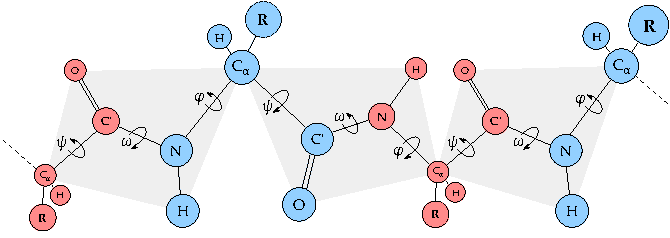
\includegraphics[width=\textwidth]{../rapport/figures/protein-torsion-angles.pdf}
    \caption{Bond angles, bond lengths and torsion angles}
    \label{fig:front}
  \end{figure}

\end{frame}

\begin{frame}[t, fragile]
  \frametitle{Protein structure}
  \framesubtitle{Measures}
\vspace{-0.5cm}
  \begin{columns}
 \column{5.5cm}
\begin{table}
  \centering
  \begin{tabular}{lrr}
    \toprule
    \multicolumn{1}{c}{Bond} & \multicolumn{1}{c}{Avg. length} & \multicolumn{1}{c}{Std.dev.} \\ \midrule 
    C-O   & 1.2260 Å & 0.0188 Å\\
    CA-C  & 1.5272 Å & 0.0191 Å\\
    N-CA  & 1.4680 Å & 0.0237 Å\\
    C-N   & 1.3234 Å & 0.0215 Å\\
    N-H   & 0.9793 Å & 0.0342 Å\\
    CA-CB & 1.5327 Å & 0.0228 Å\\
    CA-HA & 1.0747 Å & 0.0307 Å\\ \bottomrule
  \end{tabular}
  \vspace{1mm}
  \caption{Average bond lengths}
  \label{tab:average_bond_lengths}
\end{table}

\column{5.5cm}
\begin{table}
  \centering
  \begin{tabular}{lrr}
    \toprule
    \multicolumn{1}{c}{Bond} & \multicolumn{1}{c}{Avg. angle} & \multicolumn{1}{c}{Std.dev.} \\ \midrule 
    H-N-CA & $118.9553^\circ$ & $1.9979^\circ$\\
    N-CA-C & $110.6099^\circ$ & $2.4668^\circ$\\
    CA-C-O & $120.7088^\circ$ & $1.3064^\circ$\\
    CA-C-N & $116.7804^\circ$ & $1.7682^\circ$\\
    C-N-CA & $121.4547^\circ$ & $1.9946^\circ$\\
    C-N-H  & $119.5112^\circ$ & $2.1599^\circ$\\ \bottomrule
  \end{tabular}
  \vspace{1mm}
  \caption{Average bond angles}
  \label{tab:average_bond_angles}
\end{table}

\end{columns}
\end{frame}

\begin{frame}[t, fragile]
  \frametitle{RMSD}
  
\end{frame}

% Anders
\section{Backbone fitting}
\begin{frame}[t, fragile]
  \frametitle{Backbone fitting} 
%  \framesubtitle{subtitle}
\begin{center}
	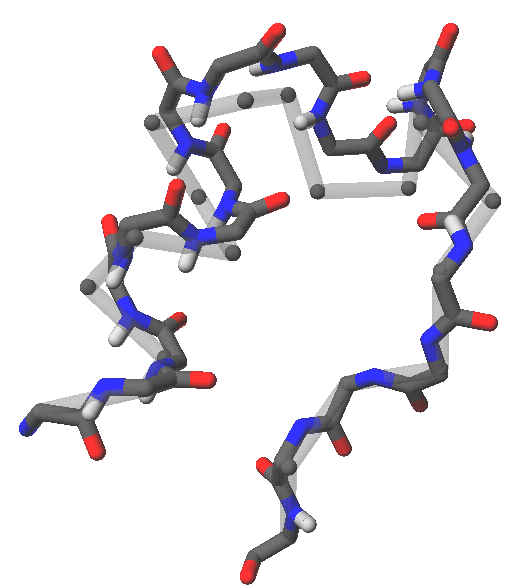
\includegraphics[width=.4\textwidth]{../rapport/figures/forside.png}
\end{center}
\end{frame}

\begin{frame}[t, fragile]
\frametitle{Backbone fitting} 
\framesubtitle{Cyclic coordinat descent}
\begin{center}
	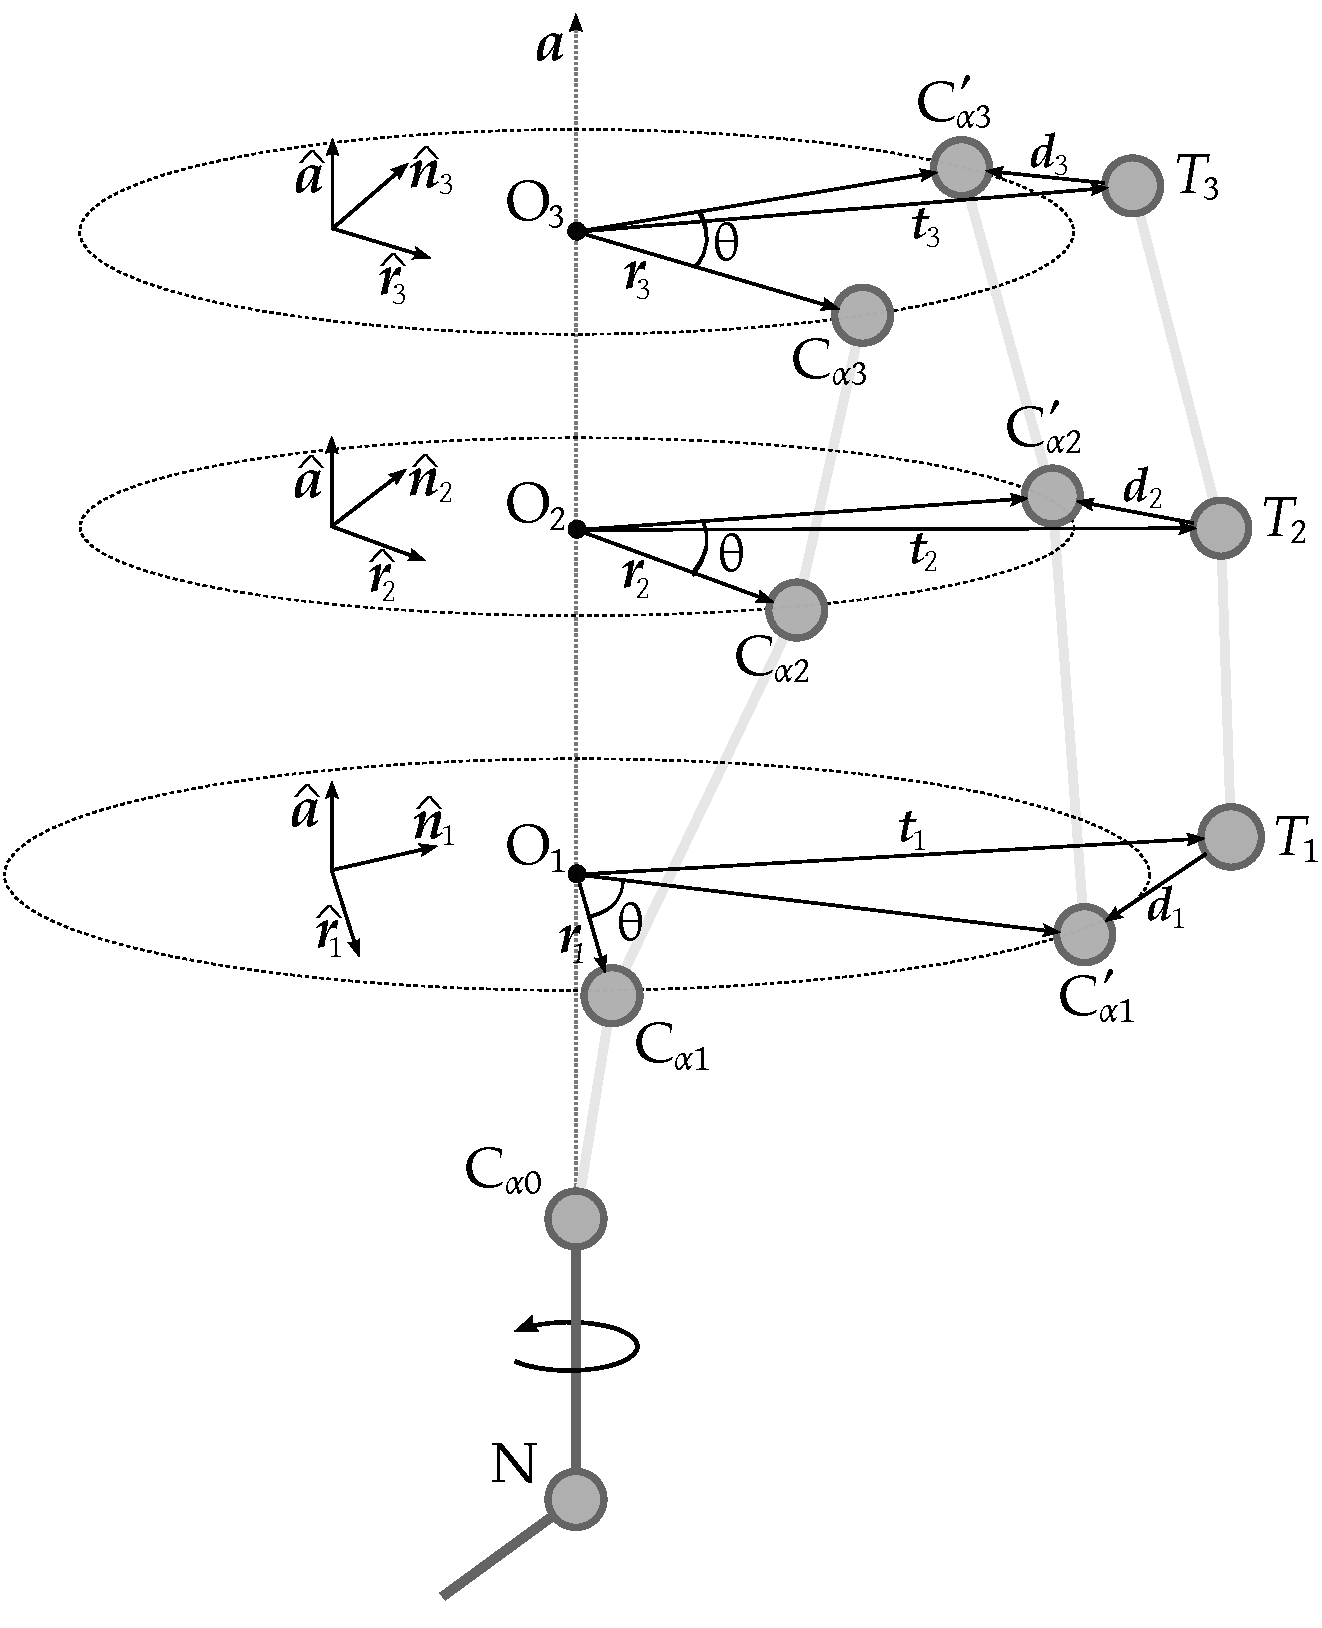
\includegraphics[width=.45\textwidth]{ccd}
\end{center}
\end{frame}

\begin{frame}[t, fragile]
\frametitle{Backbone fitting} 
\framesubtitle{Results}
\begin{columns}[c]
\column{2in}
\centering
Original\\
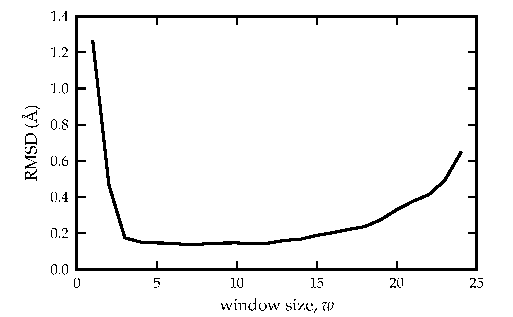
\includegraphics[width=1\columnwidth]{plot_rmsd}

\column{2in}
\centering
Fitted backbone\\
\hspace*{-.4cm}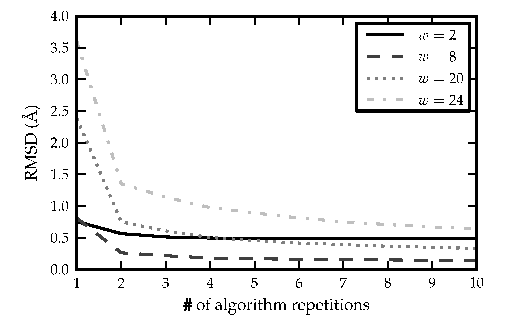
\includegraphics[width=1\columnwidth]{plot_rmsd_convergence}
\end{columns}
\end{frame}


\begin{frame}[t, fragile]
\frametitle{Backbone fitting} 
\framesubtitle{Results}
\begin{columns}[c]
\column{1.7in}
\centering
Original\\
\hspace*{-.33cm}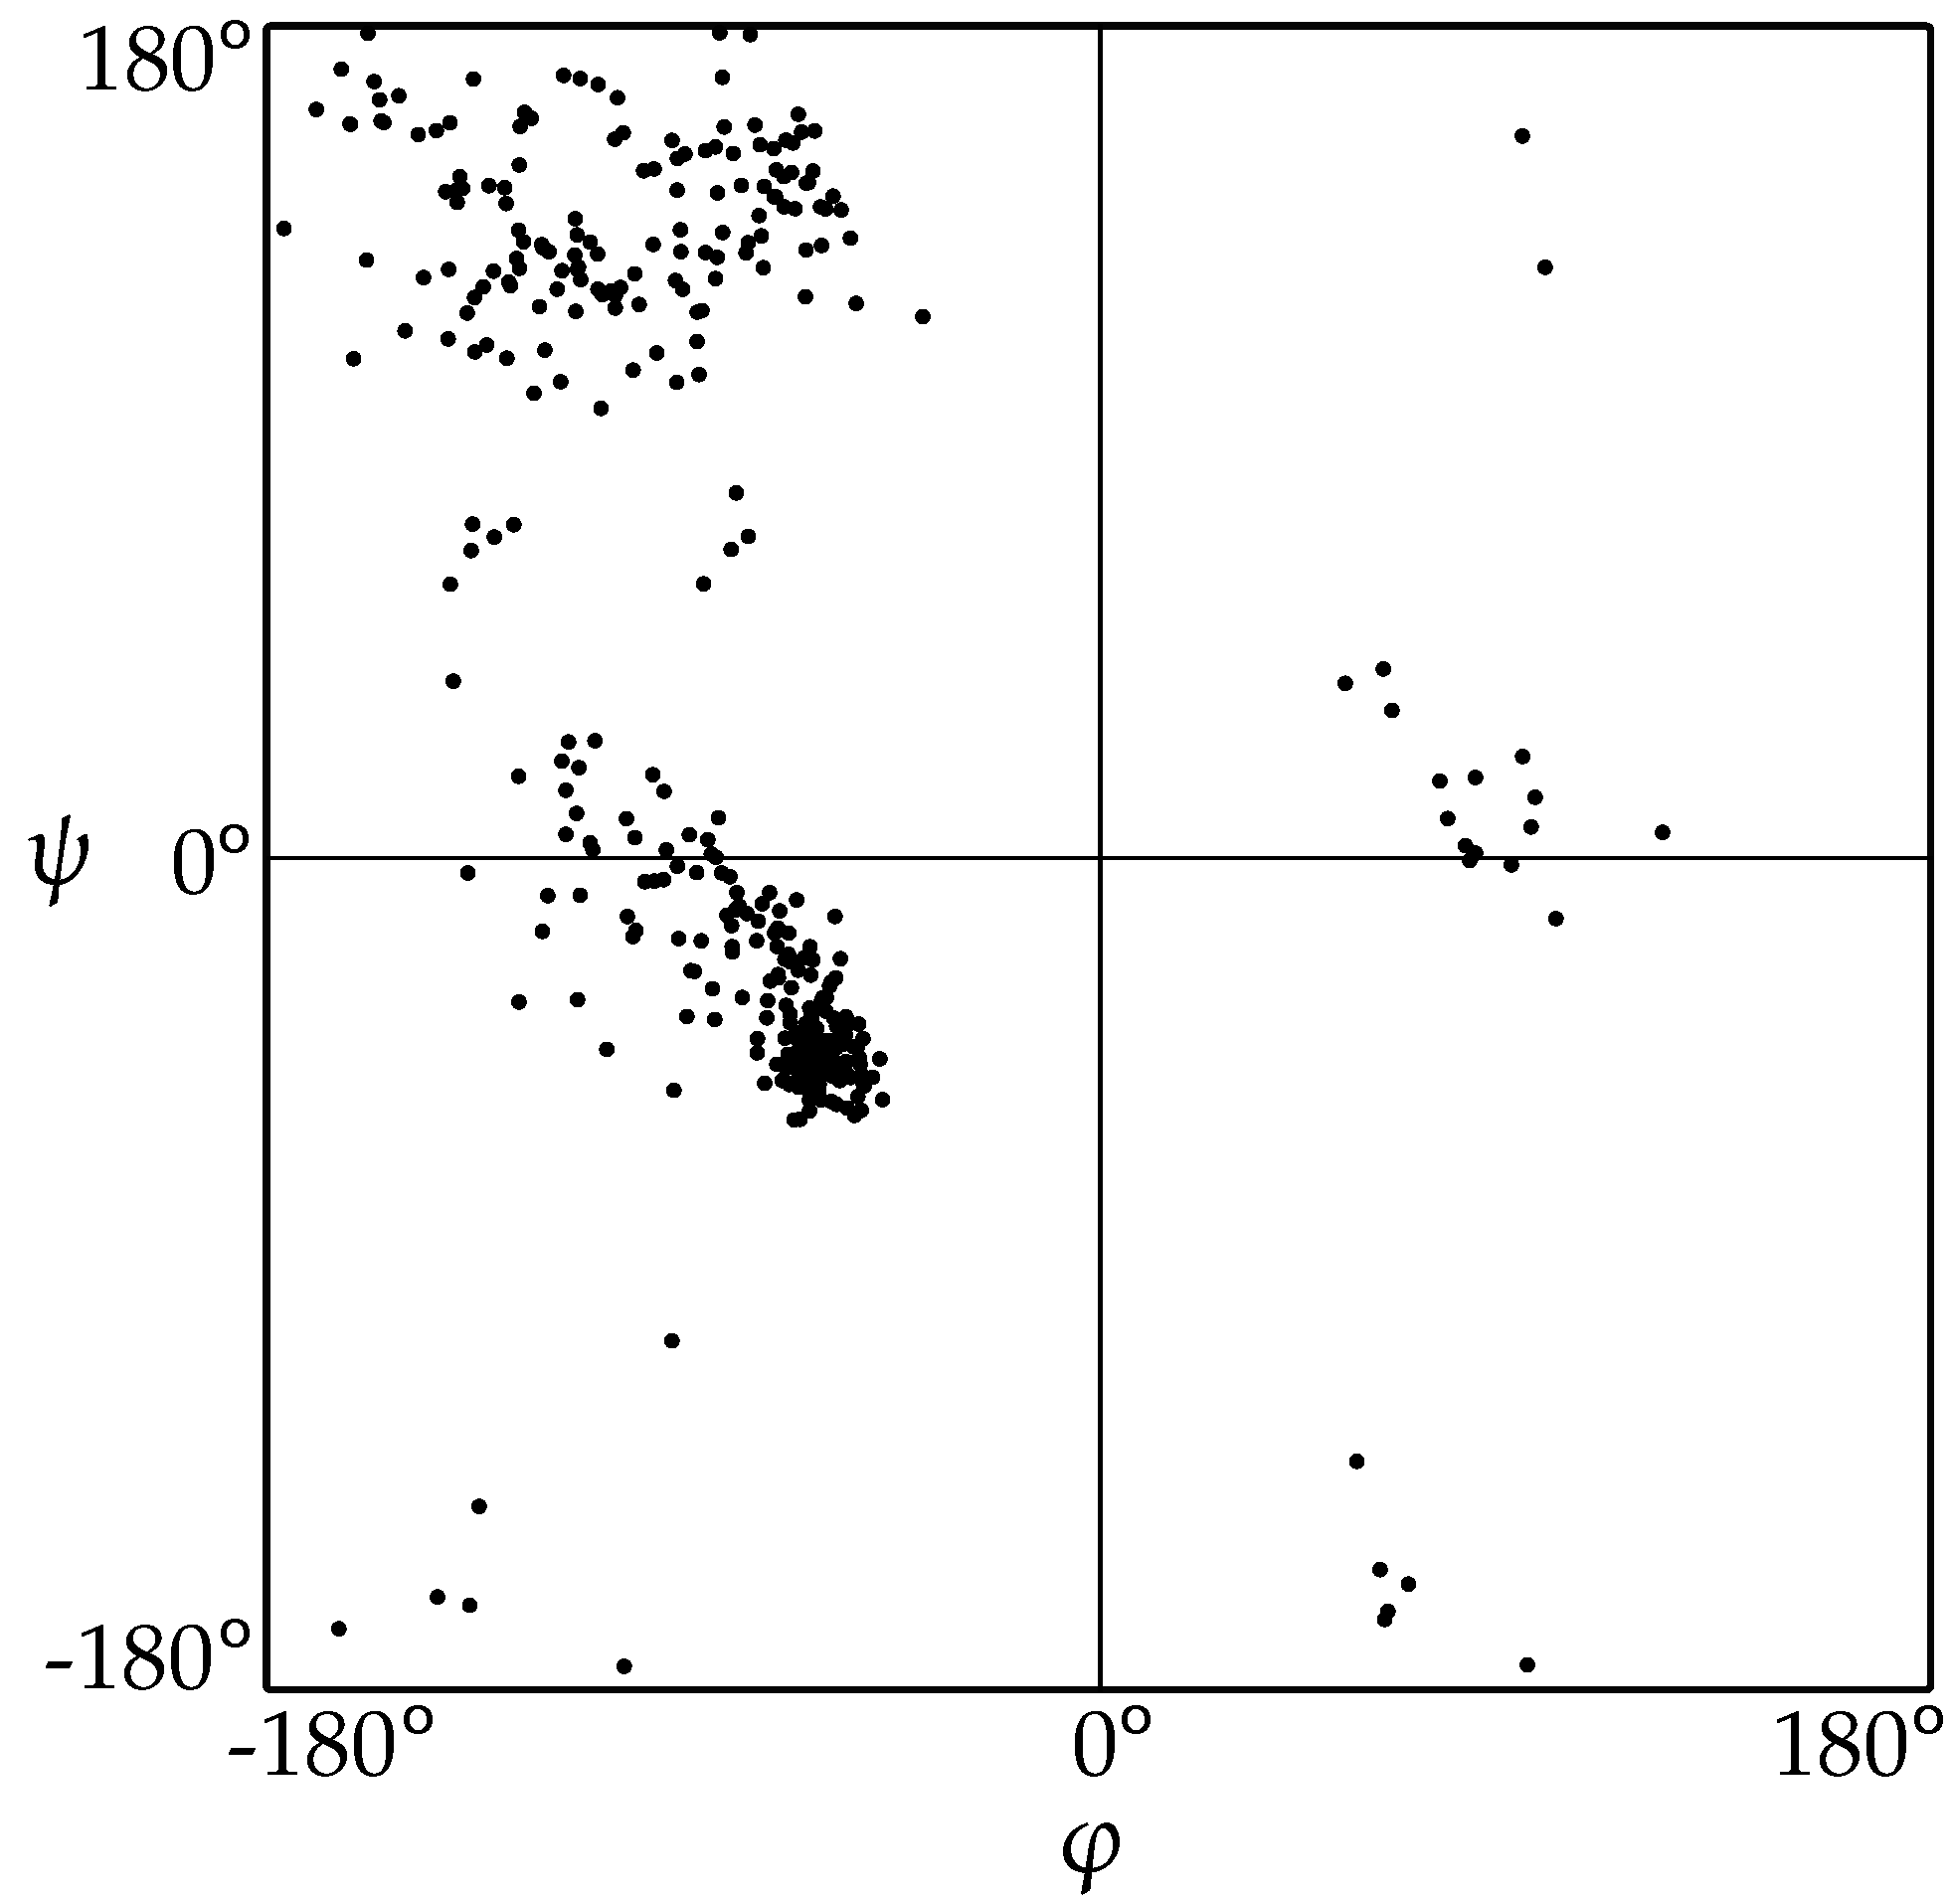
\includegraphics[width=1\columnwidth]{plot_ramachandran_orig}

\column{1.7in}
\centering
Fitted backbone\\
\hspace*{-.4cm}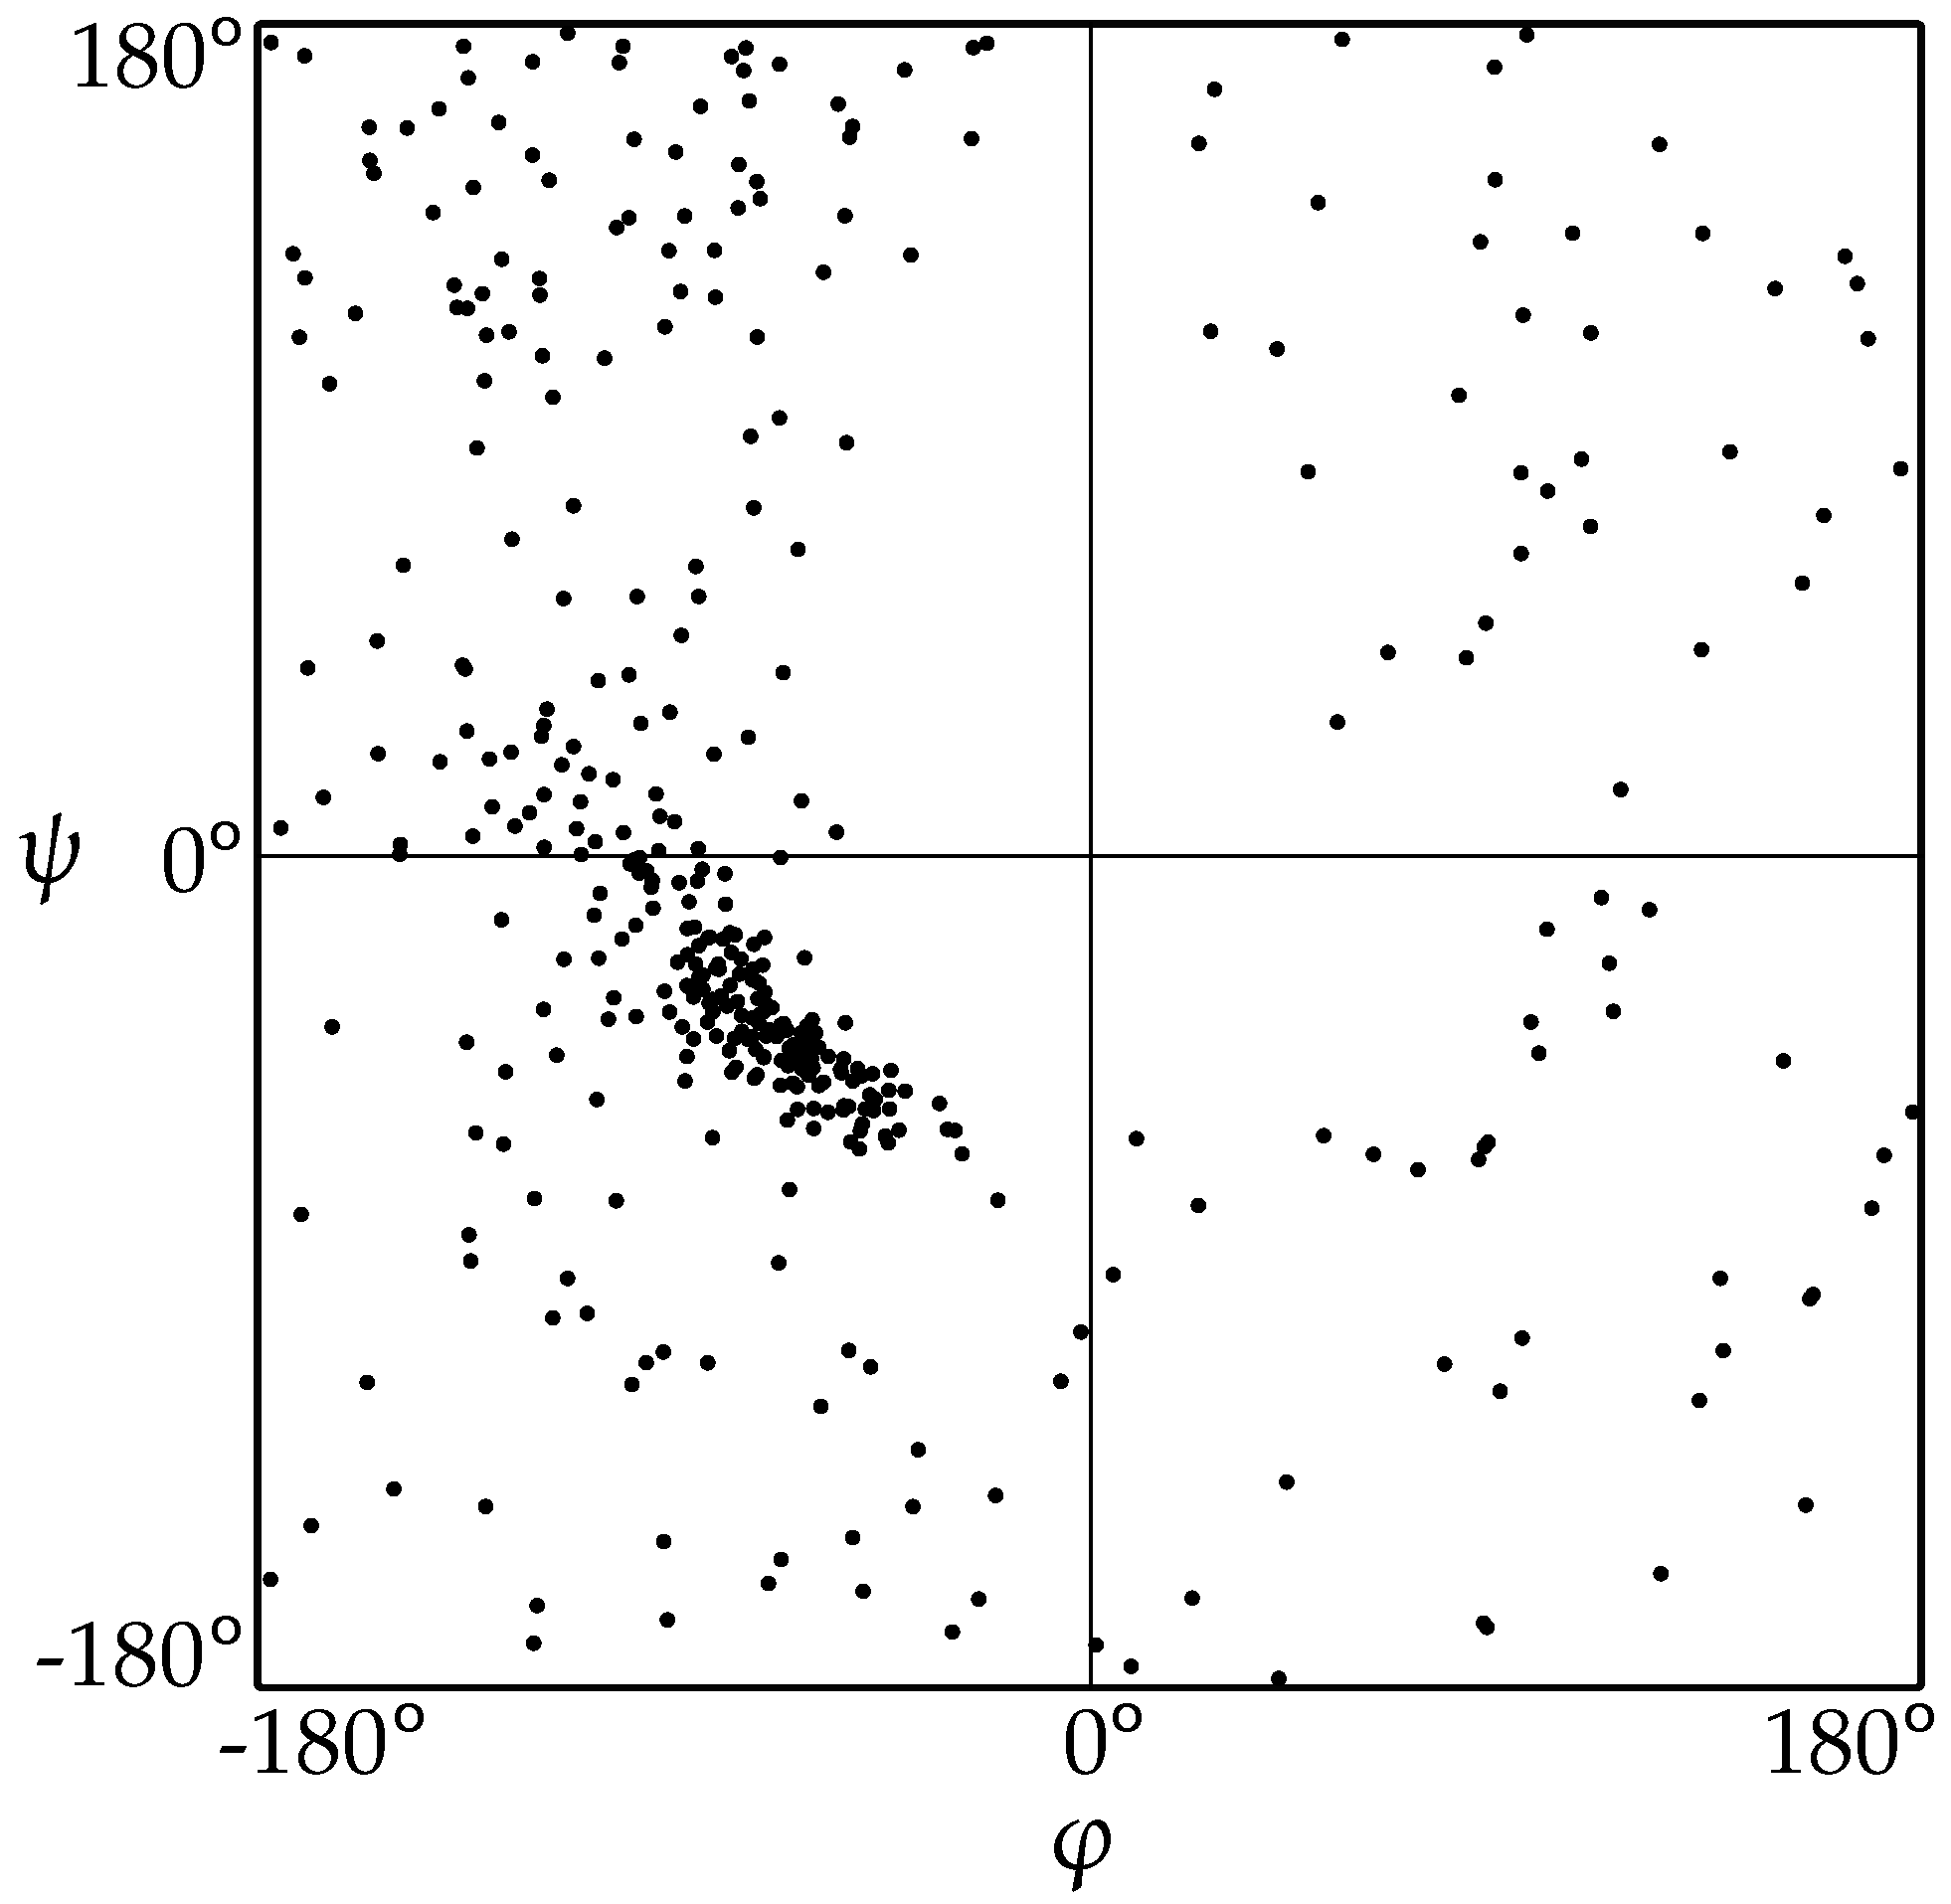
\includegraphics[width=1\columnwidth]{plot_ramachandran}
\end{columns}
\end{frame}


% Esben


\end{document}
